\documentclass[14pt]{extarticle}

\usepackage[main=russian,english]{babel}   %% загружает пакет многоязыковой вёрстки
\usepackage{fontspec}      %% подготавливает загрузку шрифтов Open Type, True Type и др.

\setmainfont{Times New Roman}
\setsansfont{Times New Roman}

\usepackage{icomma}
\usepackage{siunitx}
\usepackage[a4paper,
top=1cm,bottom=2cm,left=3cm,right=1.5cm, marginparwidth=2cm
%left=0.86cm,right=0.86cm,top=0.91cm,
]{geometry}

\usepackage{graphicx}
\usepackage{amsmath, amsfonts}
\usepackage{longtable}
\usepackage{icomma}
\usepackage{indentfirst}


\usepackage{mathrsfs}
\usepackage{xcolor}
\usepackage{hyperref}
\usepackage{enumitem}
\usepackage[export]{adjustbox}

\input{../include/definitions.inc}



\begin{document}

\begin{titlepage}
	\pagestyle{empty}




	\centering	
	\footnotesize
	МИНИСТЕРСТВО НАУКИ И ВЫСШЕГО ОБРАЗОВАНИЯ РФ\\
	НОВОСИБИРСКИЙ ГОСУДАРСТВЕННЫЙ УНИВЕРСИТЕТ\\
	Ф\,и\,з\,и\,ч\,е\,с\,к\,и\,й\, \,ф\,а\,к\,у\,л\,ь\,т\,е\,т	
	
	
	\small
	\bigskip
	\bigskip
	\bigskip
	\bigskip
	
	А.\,С.~Верещагин, А.\,В.~Мишин
	\bigskip
	
	\textbf{ТЕОРЕТИЧЕСКАЯ АЭРОГИДРОМЕХАНИКА. ЧАСТЬ 2. ПРАКТИКУМ.}
	\bigskip
	
	Учебное пособие	
	
	\vfill	
	Новосибирск\\
	2022\\


\end{titlepage}


\footnotesize

\noindent УДК \ldots \\%532.5-1/-94; 533.6.011\\
\noindent ББК \ldots \\%В253\\
\noindent В31 \ldots \\%\\


\begin{center}
	\centering
	Рецензент \ldots\\
	%зав. каф. аэрофизики и газовой динамики ФФ НГУ\\
	%акад. РАН В.\,М. Фомин\\
\end{center}


\noindent
\begin{tabular}{p{0.01\linewidth}p{0.90\linewidth}}
	& 	\textbf{Верещагин, А.\,С., Мишин, А.\,В.}\\
	\ldots %В31
	& 
	Теоретическая аэрогидромеханика. Часть 2. Практикум : учебное пособие / А.\,С. Верещагин, А.\,В.~Мишин \ldots % ; Новосиб. гос. ун-т. – Новосибирск : ИПЦ НГУ, 2021. -- 758 с.\\
\end{tabular}

\medskip
ISBN  \ldots%978-5-4437-1112-6

\medskip
Пособие представляет собой дополнение ко второй части спецкурса <<Теоретическая аэрогидромеханика>>, посвящённого введению в механику сплошных сред, включающего классические темы течения идеального газа, а также идеальной и вязкой жидкости. Спецкурс создан и читается   студентам физического факультета новосибирского государственного университета, а пособие содержит вопросы и задачи для самостоятельного решения с краткими рекомендациями.  

Предназначено для студентов математических, физических, естественнонаучных факультетов университетов, инженерно-физических и других специальностей вузов, требующих знакомство с базовыми понятиями разделов аэро- и гидродинамики, а также при подготовке к кандидатскому экзамену по специальности <<Механика жидкости, газа и плазмы>>.	

%\vfill
%\begin{flushright}
%	УДК 532.5-1/-94; 533.6.011\\
%	ББК В253\\
%\end{flushright}
%
%Рекомендовано к изданию кафедрой аэрофизики и газовой динамики ФФ НГУ (протокол №~3 от 02.10.2020 г.)
%
%\medskip	
%\noindent
%\begin{tabular}{p{0.5\linewidth}p{0.5\linewidth}}
%	& \textcopyright~Новосибирский государственный
%	университет, 2021\\
%	
%	ISBN 978-5-4437-1112-6  & \textcopyright~Верещагин А.\,С.,~2021
%	
%\end{tabular}


\newpage\normalfont\normalsize
\tableofcontents
	
\newpage
	
\section{Плоские потенциальные течения идеальной жидкости и комплексные потенциалы}



\subsection{Построение комплексного потенциала плоского потенциального течения идеальной жидкости }

Если возможно ввести систему координат так, что течение идеальной жидкости ($\rho=const$) будет описываться уравнениями:	
\begin{equation}
	\label{eq:ideal_liquid_planar_mass}
	\pd{v_x}{x}+\pd{v_y}{y} = 0,
\end{equation}
\begin{equation}
	\label{eq:ideal_liquid_planar_momentum_x}
	\pd{v_x}{t}+v_x \pd{v_x}{x} + v_y \pd{v_x}{y} = -\frac{1}{\rho} \pd{p}{x},
\end{equation}	
\begin{equation}
	\label{eq:ideal_liquid_planar_momentum_y}
	\pd{v_y}{t}+v_x \pd{v_y}{x} + v_y \pd{v_y}{y} = -\frac{1}{\rho} \pd{p}{y},	
\end{equation}
где $v_x = v_x(t,x,y)$, $v_y = v_y(t,x,y)$, $p=p(t,x,y)$ -- функции, заданные в некоторой исследуемой области, то говорят, что движение идеальной жидкости \textit{плоскопараллельное}.

\begin{dfn}
	Функция $\psi=\psi(x,y)$ такая, что 
	\[
	v_x = \pd{\psi}{y},\quad
	-v_y = \pd{\psi}{x},
	\]
	называется функцией тока. Если течение нестационарное, то $t$ -- дополнительный параметр.
\end{dfn}

Для функции $\psi = \psi(x,y)$ уравнение неразрывности (\ref{eq:ideal_liquid_planar_mass})
\[
	\pd{v_x}{x} + \pd{v_y}{y} = 
	\pd{}{x} \left( \pd{\psi}{y} \right) + \pd{}{y} \left( -\pd{\psi}{x} \right) = 0
\]
выполняется тождественно.


Рассмотрим уравнения \textit{линий тока}:
\[
	\frac{dx}{v_x(x,y)} = \frac{dy}{v_y(x,y)},
\]
тогда
\[
0 = -v_y dx + v_x dy = \pd{\psi}{x} dx + \pd{\psi}{y} dy =  d\psi.
\]
Таким образом, $\psi=\psi(x,y)$ \textit{сохраняет} одно и то же значение \textit{на линиях тока}.
		
Вектор вихря $\vec{\Omega}= \rot \vec{v}$ задается формулами:
\[
	\Omega_x = \pd{v_z}{y}-\pd{v_y}{z} = 0,\quad
	\Omega_y = \pd{v_x}{z}-\pd{v_z}{x} = 0,
\]
\[
	\Omega_z = \pd{v_y}{x}-\pd{v_x}{y} = -\pdk{\psi}{x} - \pdk{\psi}{y}.
\]
		
В случае безвихревого течения ($\vec{\Omega} = 0$):
\[
	\Delta \psi = \pdk{\psi}{x} + \pdk{\psi}{y} = 0.
\]


Если плоское течение идеальной жидкости \textit{потенциально}, тогда существует функция $\varphi(x,y)$ такая, что
\[
	v_x = \pd{\varphi}{x},\quad
	v_y = \pd{\varphi}{y}, 
\]
при этом
\begin{equation}
	\label{eq:Cauchi_Riman}
	\pd{\psi}{y} = \pd{\varphi}{x},\quad
	-\pd{\psi}{x} = \pd{\varphi}{y}.
\end{equation}
	
Иначе,
\[
\pd{\varphi}{x}\pd{\psi}{x} + \pd{\varphi}{y}\pd{\psi}{y} = 0.
\]
Отсюда следует, что линии $\varphi=const$ и $\psi=const$ \textit{ортогональны}. Такие $\varphi$ и $\psi$ называются \textit{сопряженными}.
		
	
Функции $\varphi$ и $\psi$ связаны между собой условием Коши -- Римана (\ref{eq:Cauchi_Riman}), поэтому функция комплексного переменного $w(z) = \varphi(x,y) + i \psi(x,y)$ является \textit{аналитической функцией} комплексного аргумента $z = x + i y$:
\begin{equation}
	\label{eq:complex_potential_dfn}
	w(z) = f(x+iy) = \varphi(x,y) + i  \psi(x,y).
\end{equation}

\begin{dfn}
	Функция $w(z)$ (\ref{eq:complex_potential_dfn}) называется \textit{комплексным потенциалом} плоскопараллельного потенциального течения идеальной жидкости.
\end{dfn}			
		
		
\begin{dfn}
	Комплексная функция $v(z)$, определенная по формуле
	\[
	v(z) = v_x(x,y) + i v_y(x,y),
	\] 
	называется  \textit{комплексной скоростью} (см. рис. \ref{fig:v_complex_dfn}).
\end{dfn}

Так как $w(z)$ -- аналитическая функция, то существует $dw/dz$:
\[
\od{w}{z} = \pd{\varphi}{x}+\pd{\psi}{x} i = 
\pd{\varphi}{x}-\pd{\varphi}{y} i = v_x-i v_y = v^*. 
\]

\begin{figure}
	\centering
	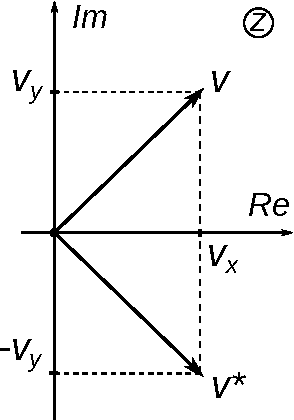
\includegraphics[width=0.3\linewidth]{../img/v_star.pdf}
	\caption{Определение комплексной скорости и её комплексно-сопряжённой величины}
	\label{fig:v_complex_dfn}
\end{figure}
					
Связь \textit{плоской потенциальной гидродинамической задачи} с теорией функций комплексного переменного (ТФКП) заключается в том, что соотношение
\[
w(z) = f(x+iy) = \varphi(x,y) + i  \psi(x,y)
\]
связывает аналитическую функцию $w(z)$ с определённой кинематической картиной течения и полем ($v_x$, $v_y$) с помощью аппарата ТФКП и наоборот.

\bigskip
Рассмотрим простейшие примеры.

\begin{problems}
\item 
\textbf{Однородное поступательное течение.}
Комплексный потенциал:
\[
	w(z) = a z,\quad
	a \in\mathbb{R}.
\]
		
Комплексная скорость:
\[
	\od{w}{z} = a = v_x - i v_y \Rightarrow
	v_x = a,\quad v_y = 0.
\]

Линии тока этого течения (при $a>0$) изображены на рис. \ref{fig:uniform_translation}.

\begin{figure}
	\centering
	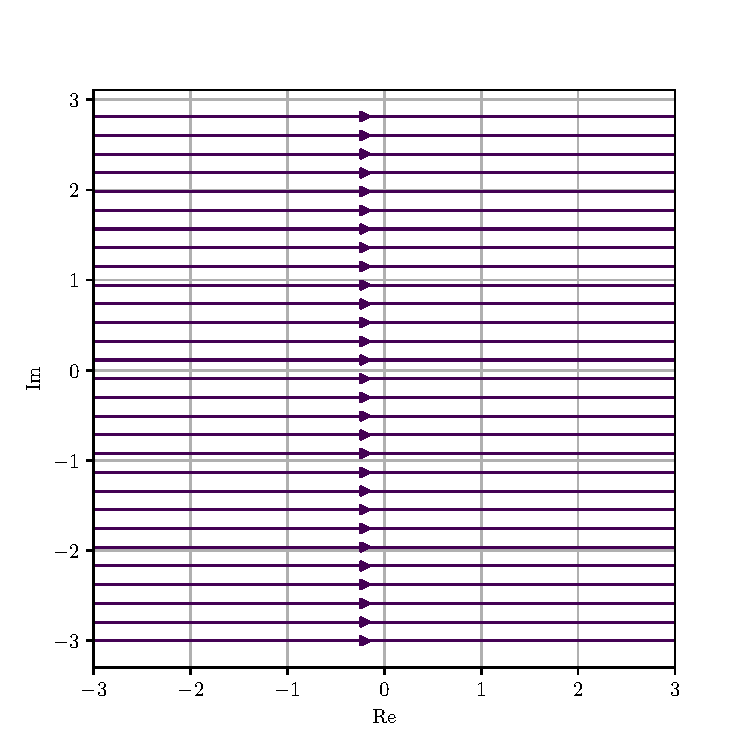
\includegraphics[width=0.45\textwidth]{../img/uniform_translation.pdf}
	\caption{Линии тока однородного поступательного движения при $a>0$}
	\label{fig:uniform_translation}
\end{figure}


\item 
\textbf{Источник и сток.} Комплексный потенциал:
\[
	w(z) = \frac{q}{2\pi}\ln(z-z_0),\quad
	q \in\mathbb{R}, z_0\in\mathbb{C}.
\]
			
Пусть $z=x+iy=re^{i\theta}$, тогда комплексная скорость (при $z_0 = 0$) имеет вид:
\[
\od{w}{z} = \frac{q}{2\pi}\frac{1}{z} \Rightarrow
\left\{
\begin{array}{l}
\displaystyle v_x = \frac{q}{2 \pi}\frac{x}{x^2+y^2} = \frac{q}{2\pi r}\cos\theta,\\
\displaystyle v_y = \frac{q}{2 \pi}\frac{y}{x^2+y^2} = \frac{q}{2\pi r}\sin\theta.
\end{array}
\right.
\]


Линии тока этого течения изображены на рис. \ref{fig:source_sink}.

\begin{figure}
	\centering
	\begin{tabular}{cc}
	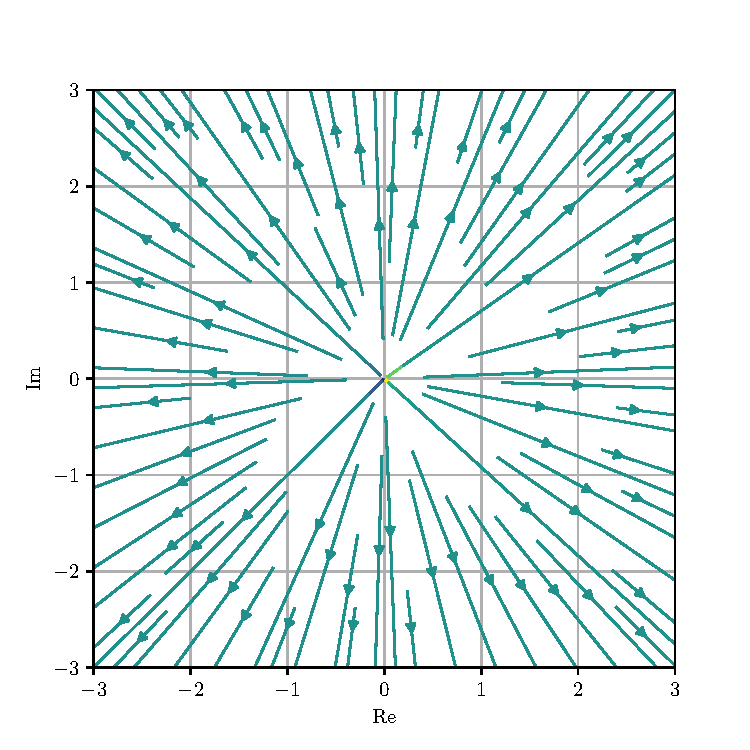
\includegraphics[width=0.45\textwidth]{../img/source.pdf} &
	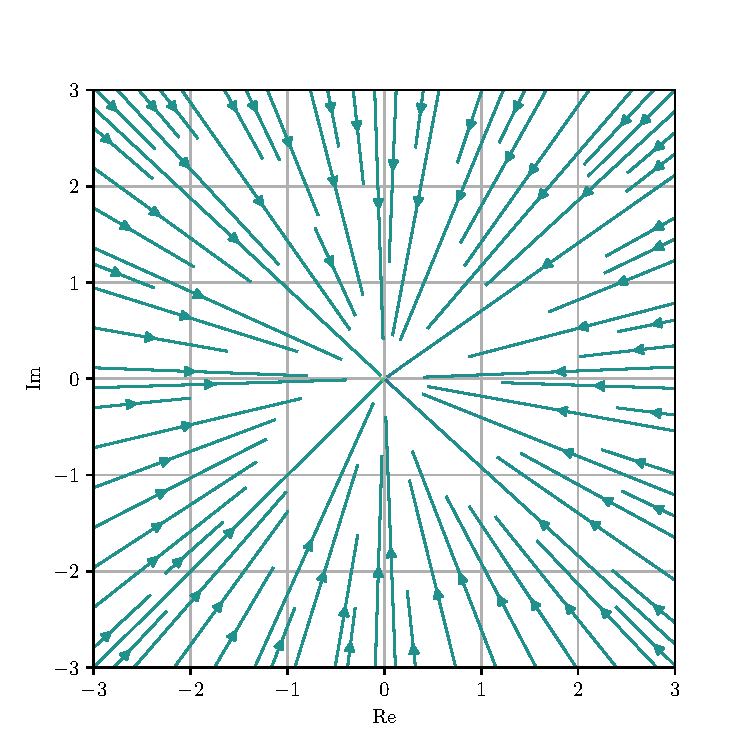
\includegraphics[width=0.45\textwidth]{../img/sink.pdf} \\
	а & б 
	\end{tabular}
	\caption{Линии тока источника ($q>0$) (a) и стока ($q<0$) (б)}
	\label{fig:source_sink}
\end{figure}

\item
\textbf{Вихрь.} Комплексный потенциал:
\[
	w(z) = \frac{\Gamma}{2\pi i}\ln(z-z_0),\quad
	\Gamma \in\mathbb{R}, z_0\in\mathbb{C}.
\]
			
Пусть $z=x+iy=re^{i\theta}$, тогда комплексная скорость (при $z_0=0$):
\[
	\od{w}{z} = \frac{\Gamma}{2\pi i}\frac{1}{z} \Rightarrow 
	\left\{
	\begin{array}{l}
		\displaystyle	v_x = -\frac{\Gamma}{2\pi}\frac{y}{x^2+y^2} = -\frac{\Gamma}{2\pi r}\sin\theta,\\
		\displaystyle	v_y = \frac{\Gamma}{2\pi}\frac{x}{x^2+y^2} = \frac{\Gamma}{2\pi r}\cos\theta.
	\end{array}
	\right.
\]

Линии тока этого течения изображены на рис. \ref{fig:rotor}.

\begin{figure}
	\centering
	\begin{tabular}{cc}
		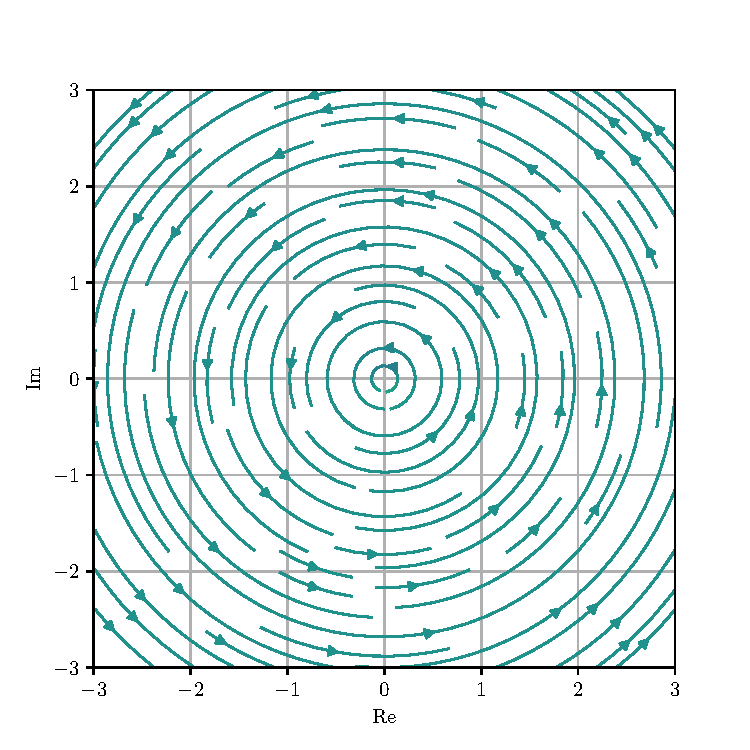
\includegraphics[width=0.45\linewidth]{../img/rot_Gamma_g_0.pdf} &
		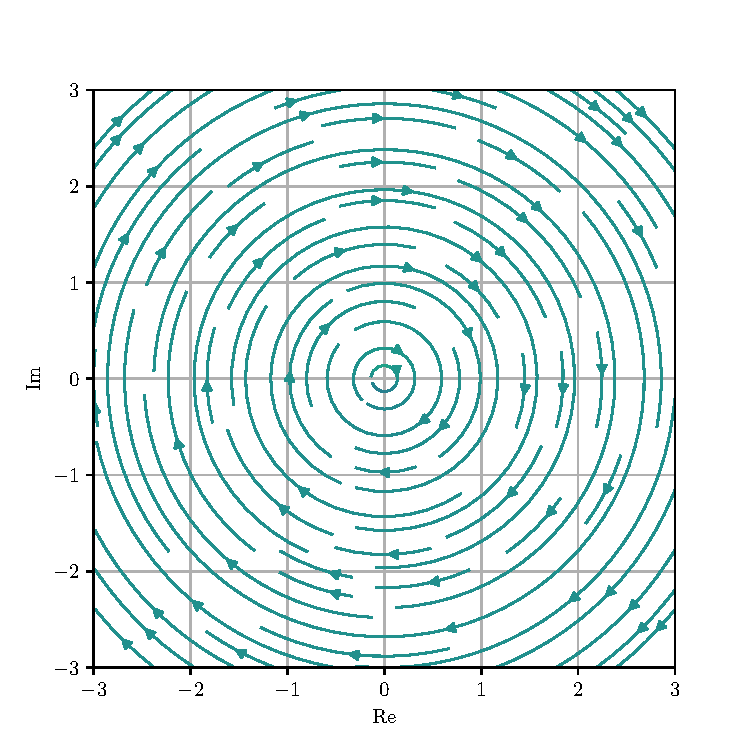
\includegraphics[width=0.45\linewidth]{../img/rot_Gamma_l_0.pdf} \\
		а & б 
	\end{tabular}
	\caption{Линии тока вихря, вращающегося в положительном ($\Gamma > 0$) (a) и отрицательном ($\Gamma < 0$) (б) направлениях}
	\label{fig:rotor}
\end{figure}

\item
\textbf{Диполь.}		
Комплексный потенциал:
\[
	w(z) = \frac{D e^{i\alpha}}{2\pi z},\quad
	D,\alpha \in\mathbb{R}.
\]
						
Пусть $z=x+iy=re^{i\theta}$, тогда комплексная скорость (при $\alpha=0$):
\[
	\od{w}{z} = -\frac{D}{2\pi}\frac{1}{z^2} \Rightarrow\displaystyle
	\left\{
	\begin{array}{l}
		v_x = -\displaystyle\frac{D}{2\pi r^2} \cos 2\theta,\\
		v_y = -\displaystyle\frac{D}{2\pi r^2} \sin 2\theta.
	\end{array}
	\right.
\]

Линии тока этого течения изображены на рис. \ref{fig:dipol}.

\begin{figure}
	\centering
	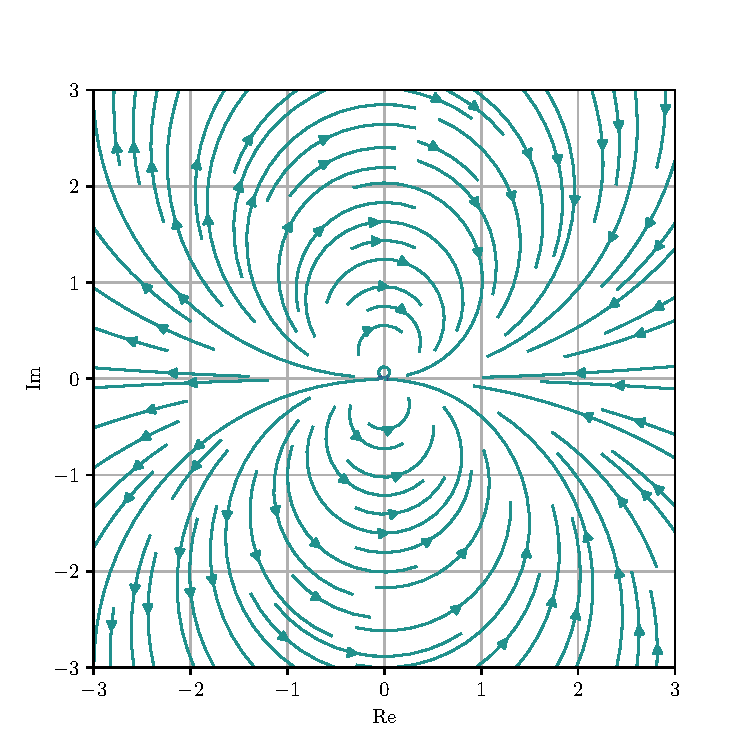
\includegraphics[width=0.45\linewidth]{../img/dipol.pdf}
	\caption{Линии тока диполя при $D>0$ и $\alpha = 0$}
	\label{fig:dipol}
\end{figure}
\end{problems}

\subsection{Построение потенциалов сложных течений}

Для моделирования течений, в которых присутствуют источники, стоки и другие элементарные течения применяется \textit{принцип суперпозиций}, заключающийся в следующем утверждении. Вследствие линейности уравнения неразрывности, если в области имеется несколько течений с потенциалами $w_1(z)$, $w_2(z)$, \ldots , $w_n(z)$, то общий потенциал всего течения в заданной точке равен сумме потенциалов всех течений, присутствующих в области:
\[
w(z) = w_1(z) + w_2(z) + \ldots + w_n(z).
\] 


Ещё один способ построения аналитических функций, описывающих плоские потенциальные течения ---  использовать \textit{метод конформных отображений} и \textit{теорему Римана о конформном отображение односвязных областей}. 

Основная идея заключается в построении конформного отображение физической плоскости $z$  на вспомогательную плоскость $\zeta$  с помощью аналитической функции $z=f(\zeta)$. Причём предполагается, что потенциал течения на вспомогательной плоскости известен $\psi(\zeta)$. Тогда искомый потенциал течения в физической плоскости  $\chi(z)$ будет выражаться из уравнений:
\[
\left\{
\begin{array}{l}
	\chi = \chi(f(\zeta)) = \psi(\zeta),\\
	z = f(\zeta).
\end{array}
\right.
\]
В этом случае комплексная скорость может быть найдена по формуле:
\[
v^* = \od{\chi}{z} = \od{\psi}{\zeta}  \od{\zeta}{z}.
\]


\subsection{Вычисление реакций и моментов сил, действующих на тело, при плоском потенциальном обтекании}
	

			
Для вычисления сил, моментов сил, действующих на выделенные контуры внутри области плоского потенциального течения, используют \textit{формулы Блазиуса -- Чаплыгина}:
\[
R^* = X - i Y = \frac{i\rho}{2} \oint\limits_C \left(\od{w}{z} \right)^2 dz,
\]	
\[
L = \Re \left[
-\frac{\rho}{2}\oint\limits_C \left(\od{w}{z} \right)^2 zdz
\right],
\]
где $R=X+i Y$ -- комплексная сила; $L$ -- величина главного момента; $\rho$ -- плотность жидкости; $C$ -- контур внутри или на границе области течения.

Также для вычисления реакций и момента главных сил можно использовать \textit{формулы Кутты -- Жуковского}. Если поток потенциален вне тела, которое можно заменить на конечное число источников, вихрей и диполей, лежащих внутри границы тела -- контура $C$, то
\[
R^* =  X - iY = i\rho\Gamma v_\infty^*,		
\]
\[
L = \Re \left[
-\rho v_\infty^*\sum\limits_{k=1}^m\Gamma_kb_k-i\rho M v_\infty^*
\right],
\]
где
$\Gamma_i$ -- циркуляции вихрей, находящихся в точках $b_i$ $(i=1,\ldots,m)$; $M$ -- суммарный момент источников и диполей; $\Gamma$ -- суммарная циркуляция вихрей, находящихся внутри тела.



\subsection{Задачи для самостоятельного решения}

\begin{problems}

	\item Установить связь функции тока  $\psi$ с линиями тока.

	\item Рассмотреть плоское течение идеальной жидкости, задаваемое комп\-лекс\-ным потенциалом $w(z) = Cz$, где $C = |C| e^{i \alpha}$.

	\item Для заданных комплексных потенциалов плоского течения идеальной жидкости:
		\begin{enumerate}
			\item 
			$
				w(z) = \ln \left( z^2 + \displaystyle\frac{1}{z^2} \right),
			$
			\item 
			$ 
			w(z) = \ln \left( 1 + \displaystyle\frac{1}{z^2} \right),
			$
		\end{enumerate}
	найти обильность $Q$ и построить качественную картину течения.
	
	\item 
	Границы какого геометрического объекта обтекаются идеальной нес\-жи\-ма\-е\-мой жидкости с заданным комплексным потенциалом
	\[
		w(z)  = v_\infty z + v_\infty \frac{R^2}{z}?
	\]
	
	Влияет ли на граничные условия добавление потенциала цир\-ку\-ля\-ции  $w(z) = \displaystyle\frac{\Gamma}{2 \pi i} \ln z$ при обтекании круга с центром в начале координат?
	
	
	\item В точках $z_1$ и $z_2$ заданы вихревые нити с циркуляциями $\Gamma_1$ и $\Gamma_2$. Требуется:
	\begin{enumerate}
		\item найти движение вихревых нитей в идеальной несжимаемой жидкости, 
		\item отдельно рассмотреть случай $\Gamma_1 = -\Gamma_2$.
	\end{enumerate}

	\item
	Какой контур обтекания соответствует комплексному потенциалу
	\[
	w(z) = z^2
	\]
	и каким будет итоговый комплексный потенциал, если в этот контур поместить источник?
	
	\item
	Идеальная несжимаемая жидкость занимает полупространство $y>0$. В точке  имеется нитевидный источник обильности $q$. Найти комплексный потенциал $w(z)$ и скорость $v(z)$ стационарного плоского течения.
	
	\item
	Найти комплексный потенциал $w(z)$ и скорость $v(z)$ стационарного плоского течения, создаваемого источником обильности $q$ при обтекании круга радиуса $R$, центр которого находится в начале координат. Источник расположен в точке $z_0$. 
	
	\item
	Пусть анализируемая 2D-система состоит из источника идеальной не\-сжимаемой жидкости обильности $q$  и непроницаемой бесконечной линии раздела, находящейся на расстоянии $h$ от источника. Найти силу, действующую на источник.
	
	\item 
	Проанализировать циркуляцию при обтекании круга идеальной не\-сжи\-маемой $2D$-жидкостью, включая описание критических точек как с графической, так и с позиции формул.
	
	\item 
	Построить потенциал обтекания эллипса на основе заданной функции отображения Жуковского $z = \zeta + c^2/\zeta$. Рассмотреть частный случай обтекания пластины.
	
	\item 
	Построить комплексный потенциал $w(z)$ обтекания непроницаемой параболы $y^2 = 2 p (x+p/2)$. Обтекание осуществляется по оси симметрии параболы $x$. Скорость на бесконечности $v_\infty$  задана.  Что за тип <<источника>> представляет член $\sqrt{pz}$? \textit{Указание: воспользоваться свойством функции тока $\psi$  на границе и формализмом распространения решения с границы на всю область.}
	
	\item
	Найти комплексный потенциал $w(z)$ и скорость $v(z)$ при стационарном потенциальном обтекании идеальной несжимаемой жидкостью угла $\alpha$. Каким будет итоговый комплексный потенциал, если в этот контур поместить источник?
	
	\item
	Определить на основе постулата Жуковского-Чаплыгина циркуляцию, возникающую при обтекании идеальной несжимаемой жидкостью пластины длиной $2l$ под углом атаки $\alpha$.
	
\end{problems}


\newpage
\section{Трёхмерные осесимметричные течения}


\subsection{Определения и постановка задачи для осесимметричных течений идеальной жидкости}



\begin{dfn}
Течение называется \alert{осесимметричным}, если существует такая прямая $l$, что во всех плоскостях, проходящих через $l$, картина течения одинакова и траектория жидкой частицы лежит в полуплоскостях, проходящих через $l$.
\end{dfn}

\begin{dfn}
Течение называется \alert{потенциальным}, если в некоторой области пространства можно определить потенциал $\varphi(t,x,y,z)$ такой, что
\[
	\vec{v} = \grad \varphi.
\]
\end{dfn}

Для трёхмерных потенциальных течений идеальной жидкости, определённых в некоторой области пространства, справедливо уравнение не\-раз\-ры\-вности:
\[
	\divo\vec{v}=\Delta\varphi = 0,\quad
	\vec{v}=\nabla \varphi
\]
и интеграл Коши
\[
	\pd{\varphi}{t} + \frac{\nabla\varphi^2}{2} + \frac{p}{\rho} = f(t)\footnote{Считаем, что поле внешних сил отсутствует.},
\]
где $p$ -- давление; $\rho$ -- плотность жидкости; $f(t)$ -- произвольная функция, определяемая из граничных и начальных условий. Интеграл Коши позволяет найти распределение давления по заданному потенциалу, известному из уравнения неразрывности ($\rho=const$).

Уравнение неразрывности в сферической системе координат ($r$,  $\lambda$, $\theta$) (рис.~\ref{fig:spherical_cylindrical_origin}а) в случае осесимметричного течения имеет вид\footnote{В следствие симметрии пренебрегли зависимостью $\varphi$ от $\lambda$.}:
\[
	\frac{1}{r^2 \sin\theta}
	\left\{
	\pd{}{r}\left( r^2 \sin\theta \pd{\varphi}{r} \right) + 
	\pd{}{\theta} \left( \sin\theta \pd{\varphi}{\theta} \right) 
%	+\pd{}{\lambda}\left( \frac{1}{\sin\theta} \pd{\varphi}{\lambda} \right)
	\right\}
	= 0,
\]
где
\[
	v_r = \pd{\varphi}{r},\quad
	v_\theta = \frac{1}{r}\pd{\varphi}{\theta}.
\]

\begin{figure}
	\centering
	\begin{tabular}{cc}
	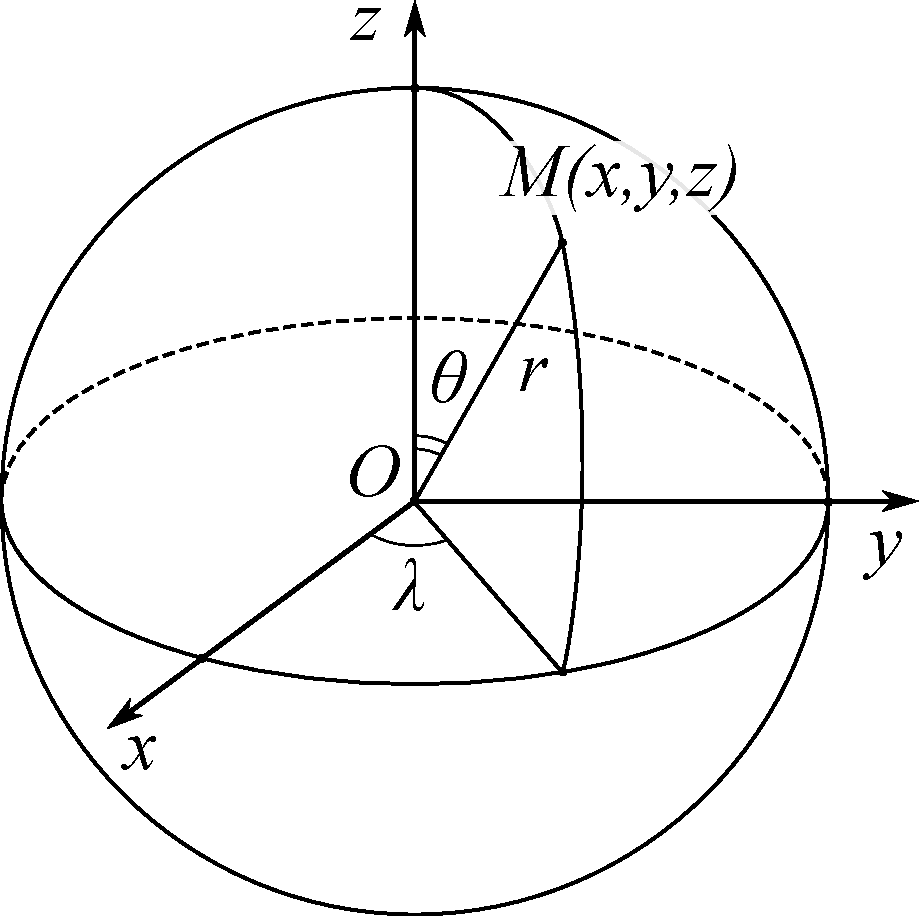
\includegraphics[width=0.45\linewidth]{../img/sphere_origin_2.pdf} & 
	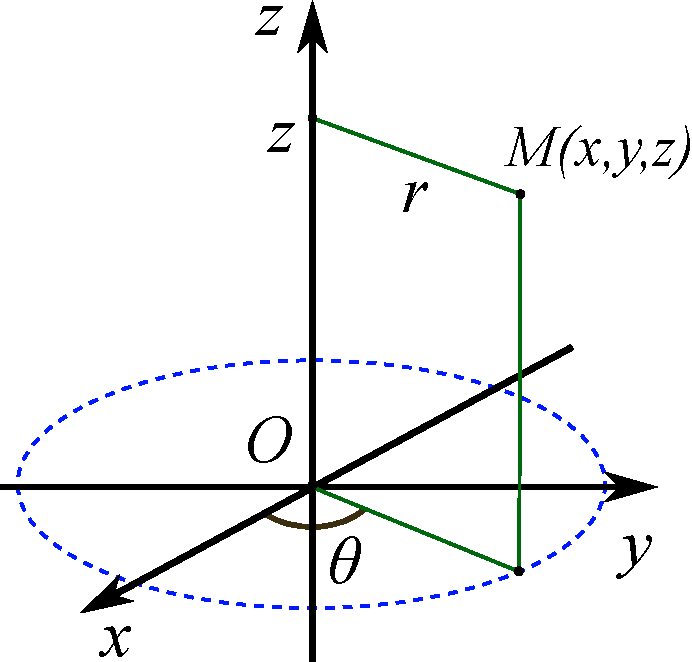
\includegraphics[width=0.4\linewidth]{../img/cylindrical_origin.pdf} \\
	а & б \\ 
	\end{tabular}
	\caption{Сферическая (а) и цилиндрическая (б) система координат}
	\label{fig:spherical_cylindrical_origin}
\end{figure}	


Уравнение неразрывности в цилиндрической системе координат ($r$, $\theta$, $z$)\footnote{В следствие симметрии пренебрегли зависимостью $\varphi$ от $\theta$.} (рис. \ref{fig:spherical_cylindrical_origin}б) в случае осесимметричного течения имеет вид:
\begin{equation}
\label{eq:mass_axis_symmetry_cylindrical}
\frac{1}{r}
\left\{
\pd{}{r}\left( r \pd{\varphi}{r} \right) + 
\pd{}{z}\left( r \pd{\varphi}{z} \right)
\right\}
= 0,
\end{equation}
где
\[
v_r = \pd{\varphi}{r},\quad
v_z =  \pd{\varphi}{z}.
\]

Из уравнение неразрывности в форме (\ref{eq:mass_axis_symmetry_cylindrical}) следует что
\[
	\pd{}{r}(r v_r)  = -\pd{}{z}(r v_z)
\]	
и существование полного дифференциала $\psi(r,z)$:
\[
	d\psi = r v_r dz - r v_z dr = \pd{\psi}{z} dz + \pd{\psi}{r} dr
\]


\begin{dfn}
Функцию $\psi\argrz$  такую, что
\[
	v_r = \displaystyle\frac{1}{r}\pd{\psi}{z},\quad
	v_z = -\displaystyle\frac{1}{r}\pd{\psi}{r},
\]
называют \alert{функцией тока для осесимметричных течений}.	
\end{dfn}

Уравнения линий тока в случае осесимметричного течения в цилиндрической системе координат:
\[
\frac{dr}{v_r} = \frac{dz}{v_z},
\]
следовательно на линиях тока:
\[
d\psi = r (v_r dz - v_z dr) = 0\quad
\Rightarrow\quad
\psi = const.
\]

Соотношения
\begin{equation}
	\label{eq:phi_psi_connection_sym}
	\pd{\varphi}{r} = \frac{1}{r}\pd{\psi}{z},\quad
	\pd{\varphi}{z} = -\frac{1}{r}\pd{\psi}{r}
\end{equation}
связывают функцию тока и потенциал для осесимметричных течений. Полученные соотношения \alert{отличаются} от условий Коши -- Римана (\ref{eq:Cauchi_Riman}), а уравнение для функции тока:
\[
	\pdk{\psi}{r}+\pdk{\psi}{z} - \frac{1}{r}\pd{\psi}{r} = 0
\]
не является уравнением Лапласа, записанным в цилиндрической системе координат. 
В случае осесимметричных течений не работают методы ТФКП. В этом случае может быть применен \alert{метод источников и стоков} и \alert{принцип суперпозиций}. 
		
Для моделирования течений, потенциалы которых известны применяется \textit{принцип суперпозиций}, заключающийся в следующем утверждении. Вследствие линейности уравнения неразрывности, если в области имеется несколько течений с потенциалами $\varphi_1(x,y)$, $\varphi_2(x,y)$, \ldots, $\varphi_n(x,y)$, то общий потенциал всего течения в заданной точке равен сумме потенциалов всех течений, присутствующих в области:
\[
\varphi(x,y) = \varphi_1(x,y) + \varphi_2(x,y) + \ldots + \varphi_n(x,y)
\] 		
или интегралу от распределенных потенциалов в некоторой области пространства.

Потенциалы и функции тока простейших осесимметричных течений в цилиндрических переменных ($r$, $z$):

\begin{enumerate}
	\item поступательное движение:
		\begin{equation}
			\label{eq:translation_3D}
			\varphi\argrz = V z \quad\Rightarrow\quad
			\psi\argrz = -\frac{V}{2}r^2 + C;
		\end{equation}
	\item  источник, сток:
		\begin{equation}
			\label{eq:source_3D}
			\varphi\argrz = -\frac{q}{4\pi} \frac{1}{\sqrt{r^2+z^2}}\quad\Rightarrow\quad
			\psi\argrz = \frac{q}{4\pi}\frac{z}{\sqrt{r^2+z^2}} + C;
		\end{equation}	
		\item диполь в направлении оси $Oz$:
			\begin{equation}
				\label{eq:dipol_3D}
				\varphi\argrz =  -\frac{M}{4\pi} \frac{z}{(\sqrt{r^2+z^2})^3}\quad\Rightarrow\quad
				\psi\argrz =  -\frac{M}{4\pi} \frac{r^2}{(\sqrt{r^2+z^2})^3}+C.
			\end{equation}
		
\end{enumerate}

\subsection{Задачи для самостоятельного решения}

\begin{problems}
	
	\item 
	Как преобразуются условия Коши-Римана в случае цилиндрических и сферических координат? Как выглядят операторы дифференциальных уравнений в постановке задач на потенциал и функцию тока (задачи Дирихле, Неймана)? 
	
	\item
	Проверить отсутствие сопротивления при стационарном равномерном прямолинейном движении шара в идеальной жидкости (парадокс Даламбера).
	
	\item Показать, что поток жидкости через поверхность, образованную вращением дуги, равен разности значений функции тока на концах этой дуги.
	
	\item Используя связь потенциала и функции тока (\ref{eq:phi_psi_connection_sym}), получить их выражения для элементарных течений, описывающих поступательное движение (\ref{eq:translation_3D}), источник (сток) (\ref{eq:source_3D}) и диполь (\ref{eq:dipol_3D}). Какое физическое значение у констант в этих формулах?
	
	\item 
	Для шара, двигающегося с ускорением в идеальной несжимаемой жидкости, определить силу, действующую на жидкость. \textit{Указание: воспользоваться уравнением Коши-Лагранжа после определения потенциала жидкости.}
	
	\item 
	Найти частоту колебаний шарика, находящегося в идеальной несжимаемой жидкости в случаях: 
	\begin{enumerate}
		\item шарик колеблется в плоскости, перпендикулярной вектору силы тяжести,
		\item шарик колеблется в поле силы тяжести.
	\end{enumerate}
	
	\item 
	Сферический пузырек всплывает в идеальной несжимаемой жидкости с плотностью $\rho$. Ускорение свободного падения $g$. Определить ускорение пузырька. Массой пузырька можно пренебречь.
	
	\item
	Сферический пузырек приводится в движение жидкостью. Ускорение жидкости вдали от пузырька равно $w$. Определить ускорение пузырька. Масса пузырька пренебрежимо мала, размер постоянен.
	
\end{problems}	


\newpage

\section{Динамика вязкой жидкости}

\subsection{Реологическое уравнение состояния вязкой жидкости}

Компоненты тензора напряжения, определяющие динамические характеристики, связаны с компонентами тензора скоростей деформаций:
\begin{equation}
\label{eq:sigma_e_connection}
\sigma = -p I + 2 \mu e,
\end{equation}
где $\sigma$ -- тензор напряжений; $\mu$ -- коэффициент динамической вязкости; $I$ --  единичный тензор; $e$ -- тензор скоростей деформации;  $p$ -- давление.

Выражение (\ref{eq:sigma_e_connection})) имеет вид:
\begin{itemize}
	\item[--] в декартовой системе координат ($x_1$, $x_2$, $x_3$):
		\[
			\sigma_{ij} = -p\delta_{ij} + 2 \mu e_{ij}\quad (i,j = 1,2,3),	
		\]
		где
		\[
			\delta_{ij} = 
			\left\{
			\begin{array}{cl}
				1, & i = j,\\
				0, & i \neq j,\\
			\end{array}
			\right.\quad
			e_{ij} = \frac{1}{2}\left(
			\pd{v_i}{x_j}+\pd{v_j}{x_i}
			\right)
		\]
		\[
			(i,j = 1,2,3);
		\]
		
	\item[--] в сферической системе координат ($r$, $\lambda$, $\theta$) (рис. \ref{fig:spherical_cylindrical_origin}а):
	\[
	\sigma_{rr} = -p +2\mu\pd{v_r}{r},\quad 
	\sigma_{\lambda\lambda} = -p + 2\mu 
	\left(
		\frac{1}{r\sin\theta} \pd{v_\lambda}{\lambda} + \frac{v_r}{r} + \frac{v_\theta \ctg\theta}{r}
	\right),
	\]
	\[
	\sigma_{\theta\theta} = -p + 2\mu \left(
	\frac{1}{r} \pd{v_\theta}{\theta} + \frac{v_r}{r}
	\right),
	\]
	\[
	\begin{array}{l}
	\sigma_{r\theta} = \sigma_{\theta r} = \displaystyle \mu\left(
	\frac{1}{r} \pd{v_r}{\theta} + \pd{v_\theta}{r} - \frac{v_\theta}{r}
	\right), \\
	\sigma_{\lambda\theta} =  \sigma_{\theta\lambda}= \displaystyle \mu \left(
	\frac{1}{r\sin\theta} \pd{v_\theta}{\lambda} + \frac{1}{r}\pd{v_\lambda}{\theta} - \frac{v_\lambda \ctg\theta}{r}
	\right),\\
	\sigma_{\lambda r} =  \sigma_{r\lambda}= \displaystyle \mu \left(
	 \pd{v_\lambda}{r} + \frac{1}{r\sin\theta}\pd{v_r}{\lambda} - \frac{v_\lambda}{r}
	\right);
	\end{array}
	\]
	
	\item[--] в цилиндрической системе координат ($r$, $\theta$, $z$) (рис.~\ref{fig:spherical_cylindrical_origin}б):
	\[
	\sigma_{rr} = -p + 2 \mu \pd{v_r}{r},\quad
	\sigma_{\theta\theta} = -p + 2\mu \left( \frac{1}{r} \pd{v_\theta}{\theta} +\frac{v_r}{r} \right),\quad
	\sigma_{zz} = -p + 2\mu \pd{v_z}{z},
	\]
	\[
	\begin{array}{l}
		\sigma_{r\theta} = \sigma_{\theta r} = \displaystyle \mu\left(
		\frac{1}{r} \pd{v_r}{\theta} + \pd{v_\theta}{r} - \frac{v_\theta}{r}
		\right), \\
		\sigma_{\theta z} =  \sigma_{z\theta}= \displaystyle \mu \left(
		 \pd{v_\theta}{z} + \frac{1}{r}\pd{v_z}{\theta} 
		\right),\\
		\sigma_{zr} =  \sigma_{rz}= \displaystyle \mu \left(
		\pd{v_z}{r} + \pd{v_r}{z}
		\right).
	\end{array}
	\]
\end{itemize}

Для вычисления равнодействующей силы $\vec{F}$, со стороны вязкой жидкости на тело, ограниченное поверхностью $S$, необходимо вычислить следующий интеграл:
\[
\vec{F} = \int\limits_S \vec{n} \cdot \sigma \, dS,
\]
где $\vec{n}$ -- вектор внешней единичной нормали к поверхности $S$.


\subsection{Основные уравнения вязкой жидкости}

Движение вязкой несжимаемой жидкости описывается \alert{уравнениями Навье -- Стокса}:
\begin{equation}
	\label{eq:navier–stokes_mass}
	\divo \vec{v} = 0,
\end{equation}
\begin{equation}
	\label{eq:navier–stokes}
	\pd{\vec{v}}{t} + (\vec{v}\cdot\nabla)\vec{v} = -\frac{1}{\rho}\nabla p + \nu \Delta \vec{v} + \vec{f},
\end{equation}
где \alert{неизвестные функции}: $\vec{v}\argtxv$ -- вектор скорости; $p\argtxv$ -- давление; $T\argtxv$~-- температура. \alert{Константы и заданные зависимости}, определяющие течение: $\rho$ -- плотность; $\nu=\mu/\rho$ -- коэффициент кинематической вязкости; $\vec{f}$ -- вектор внешних сил. 
		
Расчёт температурного поля, если требуется осуществляется путём решения дополнительного уравнения, с использованием решения уравнений Навье-Стокса:
\[
c_V\left(\pd{T}{t} + (\vec{v}\cdot\nabla)T \right) = \frac{\kappa}{\rho} \Delta T + \frac{2\mu}{\rho} e_{ij}e_{ij},
\]
\[
e_{ij} = \frac{1}{2}\left(
\pd{v_i}{x_j}+\pd{v_j}{x_i}
\right)\quad
(i,j = 1,2,3),
\]
где $e_{ij}$ -- тензор скоростей деформации ($i,j = 1,2,3$); $\kappa$ -- коэффициент температуропроводности.

В случае \alert{осесимметричного течения} уравнения Навье-Стокса имеют вид:
\begin{itemize}
	\item[--] в цилиндрической системе координат ($r$, $\theta$, $z$) (рис. \ref{fig:spherical_cylindrical_origin}б) \footnote{Пренебрегли зависимостью от $\theta$.}:
\[
\pd{}{r} (r v_r) + \pd{}{z} (r v_z) = 0,
\]
\[
\pd{v_r}{t} + v_r\pd{v_r}{r} + v_z\pd{v_r}{z} = -\frac{1}{\rho} \pd{p}{r} + \nu \left(\Delta v_r - \frac{v_r}{r^2}\right),
\]
\[
\pd{v_z}{t} + v_r\pd{v_z}{r} + v_z\pd{v_z}{z} = -\frac{1}{\rho} \pd{p}{z} + \nu \Delta v_z,
\]
\[
\Delta = \pdk{}{r}+\frac{1}{r}\pd{}{r} + \pdk{}{z};
\]
	\item[--] в сферической системе координат ($r$,  $\lambda$, $\theta$) (рис. \ref{fig:spherical_cylindrical_origin}а)\footnote{Пренебрегли зависимостью от $\lambda$.}:
\[
\frac{1}{r^2} \pd{}{r}(r^2 v_r) + \frac{1}{r \sin \theta} \pd{}{\theta}(v_\theta \sin\theta) = 0,
\]
\[
\pd{v_r}{t} + v_r\pd{v_r}{r} + \frac{v_\theta}{r} \pd{v_r}{\theta} - \frac{v_\theta^2}{r} = -\frac{1}{\rho} \pd{p}{r} + 
\nu \left(\Delta v_r - \frac{2 v_r}{r^2} - \frac{2}{r^2}\pd{v_\theta}{\theta} - \frac{2 v_\theta \ctg\theta}{r^2}\right),
\]
\[
\pd{v_\theta}{t} + v_r\pd{v_\theta}{r} + \frac{v_\theta}{r} \pd{v_\theta}{\theta} + \frac{v_r v_\theta}{r} = 
-\frac{1}{r \rho} \pd{p}{\theta} + 
\nu \left(\Delta v_\theta + \frac{2}{r^2}\pd{v_r}{\theta} - \frac{v_\theta}{r^2 \sin^2 \theta}\right),
\]
\[
\Delta = \frac{1}{r^2} \pd{}{r}\left(r^2\pd{}{r}\right) + \frac{1}{r^2 \sin\theta} \pd{}{\theta} \left(\sin\theta \pd{}{\theta}\right).
\]
\end{itemize}

\subsection{Постановка граничных условий в контактных задачах вязкой жидкости}

При исследовании обтекания твёрдых тел вязкой жидкостью необходимо использовать условие \alert{прилипания}, заключающееся в том, что скорость жидкости на границе с телом совпадает со скоростью перемещения границы. Если тело покоится, то скорость жидкости равна нулю.

На \alert{контактном разрыве} необходимо также ставить динамическое ус\-ло\-вие, заключающееся в равенстве напряжений, возникающих на касательной к разрыву площадке.

Для течения вязкой жидкости и идеального газа (рис.~\ref{fig:viscous_fluid_gas}) без учёта сил поверхностного натяжения ставятся следующие условия.

\alert{Кинематическое} условие:
\[
v_n|_S = u_n,
\]
где $S$ -- поверхность контактного разрыва; $v_n$ -- нормальная составляющая скорости жидкости на границе; $u_n$ -- нормальная составляющая скорости газа на границе; $\vec{n}$ -- вектор нормали к поверхности.

\alert{Динамические} условия:
\[
(\vec{n}\cdot\sigma)\cdot\vec{n}|_S= p|_S = p_0,
\]
\[
(\vec{n}\cdot\sigma)\cdot\vec{\tau}|_S = 0,
\]
где $\sigma$ -- тензор напряжений в вязкой жидкости; $p_0$ -- давление газа; $\vec{\tau}$ -- касательный вектор к поверхности.

\begin{figure}
	\centering
	\begin{tabular}{c}
		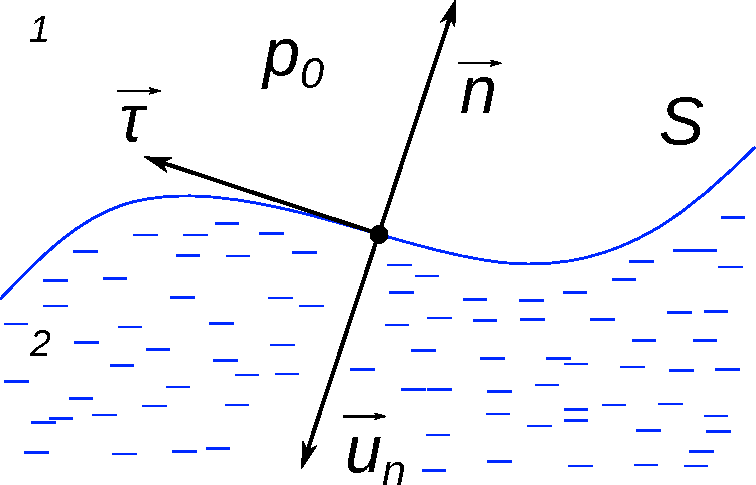
\includegraphics[width=0.6\linewidth]{../img/free_bound} \\
	\end{tabular}
	\caption{Пример течения с контактным разрывом для вязкой жидкости и идеального газа: 1 -- идеальный газ; 2 -- вязкая жидкость}
	\label{fig:viscous_fluid_gas}
	
\end{figure}	

\subsection{Коэффициенты подобия при течениях вязкой несжимаемой жидкости}

Используя замену переменных 
\[
t = T t',\quad
x = L x',\quad 
y = L y',\quad
z = L z',			
\]
\[
\vec{v}\argtxyz = V \vec{v}'\argtxyztick,\quad
\vec{f}\argtxyz = F \vec{f}'\argtxyztick
\]
\[
p\argtxyz = P p\argtxyztick',
\]
где $T$, $L$, $V$, $P$, $F$ -- характерные значения времени, размера течения, скорости, давления, силы сплошной среды, а штрихованные параметры -- это новые безразмерные переменные, уравнения Навье-Стокса (\ref{eq:navier–stokes}) приводится к следующему виду:
\begin{equation}
\label{eq:Navier-Stokes_dim}
\Sh\pd{\vec{v'}}{t'} + (\vec{v}' \cdot \nabla') \vec{v'} = \frac{1}{\Fr} \vec{f'}  - \Eu \nabla' p' + 
\frac{1}{\Re} \Delta' \vec{v}',
\end{equation}
где $\nabla'$ и $\Delta'$ -- операторы градиента и Лапласа по штрихованным переменным.

\begin{dfn}
		Безразмерные комплексы, обуславливающие течения вязкой жидкости, являются критериями подобия и имеют следующие названия:
		\[
		\begin{tabular}{ll}
			$\displaystyle\frac{L}{VT} = \Sh$ -- число Струхаля, & $\displaystyle\frac{P}{\rho V^2}=\Eu$ -- число Эйлера, \\
			$\displaystyle\frac{VL}{\nu} = \Re$ -- число Рейнольдса, & $\displaystyle\frac{V^2}{F L}=\Fr$ -- число Фруда.
		\end{tabular}
		\]
\end{dfn}

Число Струхаля $\Sh$ определяет насколько течение можно считать установившимся (стационарным), число Рейнольдса $\Re$~-- вклад  вязких членов по сравнению с инерционными, число Эйлера $\Eu$~-- вклад градиента давления по сравнению с напором, число Фруда $\Fr$~-- вклад внешнего поля.

\subsection{Приближение Стокса и ползущие течения}

\begin{dfn}
Течения, для которых число Рейнольдса много меньше $1$:
\[
	\Re= \frac{L V \rho}{\mu} \ll 1,
\]
называются ползущими течениями.
\end{dfn}

Произведём оценку вклада конвективного слагаемого по сравнению с вязким в уравнениях Навье -- Стокса (\ref{eq:navier–stokes}) для ползущего течения:
\[
\frac{\rho |(\nabla\cdot\vec{v})\vec{v}| }{\mu |\Delta\vec{v}|} \sim 
\frac{\rho V^2}{L} : \frac{\mu V }{(L)^2} = \Re \ll 1.
\]

Отбрасывая \alert{нелинейные инерционные члены} $(\nabla\cdot\vec{v})\vec{v}$ в (\ref{eq:navier–stokes}), получим линейное приближение \alert{Стокса} уравнений (\ref{eq:navier–stokes_mass}), (\ref{eq:navier–stokes}):
\begin{equation}
\label{eq:Stokes}
\divo \vec{v} = 0,\quad
\nabla p = \mu \Delta\vec{v}.
\end{equation}
	
\subsection{Задачи для самостоятельного решения}

\begin{problems}
	
	\item 
	При течении вязкой жидкости между двумя параллельными плоскостями найти силу, действующую на единицу длины каждой из плоскостей. Аналогично, найти силу, действующую на единицу длины, при течении вязкой жидкости в цилиндре. 
	
	\item 
	Определить скорость вязкой жидкости при стационарном ламинарном течении по наклонной плоскости (плоскость образует угол $\alpha$ с горизонтом). Толщина слоя жидкости $h$.
	
	\item 
	Найти скорость $v$ вязкой жидкости с вязкостью $\mu$ при течении между двумя цилиндрами радиуса $R_1$ и $R_2$ ($R_2>R_1$) при условии, что внутренний цилиндр вращается с частотой $\omega_1$, а внешний -- с частотой $\omega_2$.
	

	
	\item 
	Найдите вектор скорости, давление, вектор вихря и силу Стокса при обтекании шара вязкой жидкостью в приближении Стокса.
	
	{\small
	\textit{Указание.}	
	
	Решение (поиск констант) предлагается искать следующим образом: подействуйте ротором на уравнение количества движения в приближении Стокса, что приведёт к уравнению на вектор вихря, затем воспользуйтесь соображением симметрии для вектора вихря, далее, найдите вектор вихря с точностью до константы, решая дифференциальное уравнение, затем, пользуясь уравнением неразрывности и разложением в ряд для скоростей в сферических координатах (по расстоянию от центра шара), найдите компоненты скоростей с учетом граничного условия. Определив давление, найдите силу Стокса.  \newline		
	Решение  также можно искать следующим образом. Подействуйте оператором дивергенции на уравнение количества движения с целью выделения уравнения на давление. Это даст множество решений, но из лекции мы знаем какое взять. Почему член $1/r$ не входит в выражение для давления? Помимо условий на границе шара, используйте уравнение неразрывности для получения условий на неизвестные константы. При нахождении констант не забудьте также про константу при давлении. Почему член $1/r^3$ не входит в выражение для скорости? Почему член $1/r$  входит в выражение для скорости и к чему это приводит (относительно обтекания сферы идеальной жидкостью посмотреть)? Как симметрия задачи оказывает влияние на составление членов, потенциально подходящих под решение?
	}

	\item 
	Проанализировать поведение найденного поля скоростей при отдалении от шара. Почему наблюдается такое поведение скоростей? Что следует сделать, чтобы уточнить полученное решение? 
	
	\item
	Показать, что в вязкой жидкости происходит диссипация энергии.
	 
	{\small \textit{Указание:} показать, что работа, совершаемая над жидкостью, не целиком идёт на изменение кинетической энергии.}

\end{problems}

\newpage

\section{$\Pi$-теорема}

\subsection{Определения и примеры}

\begin{dfn}
	Два физических явления называются \alert{подобными}, если величины, характеризующие одно явление, могут быть получены из соответствующих величин другого, взятых в сходственных пространст\-вен\-но-вре\-мен\-ных точках, простым умножением на \textit{одинаковые во всех точках множители}, называемые \textit{коэффициентами подобия}.
\end{dfn}

Примером подобия может служить система уравнений Навье-Стокса, записанная в безразмерных переменных (\ref{eq:Navier-Stokes_dim}). Критериями подобия являются безразмерные комплексы: число Рейнольдса $\Re$, число Фруда $\Fr$, число Струхаля $\Sh$, число Эйлера $\Eu$. Все обезразмеренные решения уравнений (\ref{eq:navier–stokes}) будут являться функциями от этих безразмерных комплексов.

Для того чтобы использовать теорию размерности необходимо ввести понятие \alert{размернооднородной} функции. 

\begin{dfn}
	Функция $f(x_1, x_2, \ldots, x_n)$ называется \alert{размернооднородной}, если существует такая совокупность чисел $b_k$ ($k=\overline{1,m}$), что имеет место равенство
	\begin{equation}
	\label{eq:dimension_uniform_function_dfn}
	f(\alpha_1^{a_{11}}\ldots \alpha_m^{a_{1m}}x_1,\ldots,
	\alpha_1^{a_{n1}}\ldots \alpha_m^{a_{nm}}x_n) = 
	\alpha_1^{b_1}\alpha_2^{b_2}\ldots \alpha_m^{b_m} f(x_1, x_2, \ldots, x_n)
	\end{equation}
	для всех $\alpha_k$ ($k=\overline{1,m}$) и $x_i$ ($i=\overline{1,n}$) в области определения.
\end{dfn}

Рассмотрим классическую задачу колебания математического маятника, представляющего собой механическую систему, состоящую из материальной точки на конце невесомой нерастяжимой нити или лёгкого стержня и находящуюся в однородном поле сил тяготения. Известно, что период его \alert{малых} колебания определяется формулой:
\[
T(l, g) = 2 \pi \sqrt{\frac{l}{g}},
\]
где $T$ -- период колебания, с; $l$ -- длина, м; $g$ -- ускорение свободного падения, м/с$^2$.

Пусть длина нити $l = x_1$~м, ускорение свободного падения $g = x_2$~м/c$^2$. Коэффициенты $\alpha_i$ ($i=1,2$) -- это коэффициенты пересчёта параметров из одной системы единиц в другую (например, связанной с метрами и секундами в систему единиц, связанную с километрами и минутами, т.е. $\alpha_1 = 10^{-3}$~км/м, $\alpha_2 = 60^{-1}$~мин/с).

Период колебаний маятника $T$ является размернооднородной функцией, т.к. равенство
\begin{equation}
\label{eq:T_dim_connection}
T(\alpha_1 x_1, \alpha_1 \alpha_2^{-2} x_2) = 2 \pi \sqrt{\frac{\alpha_1 x_1}{\alpha_1 \alpha_2^{-2} x_2}} = \alpha_2 T(x_1, x_2)
\end{equation}
выполнено для всех $x_i$, $\alpha_j$ ($i,j=1,2$) в области определения. В данном случае $b_1 = 0$, $b_2 = 1$. 

Для указанных значений $\alpha_i$ выражение (\ref{eq:T_dim_connection}) связывает период колебания маятника в часах, через параметры выраженные в системе единиц СИ.

Вообще говоря, любая функция, связывающая параметры явления, с корректным приведением размерностей является размерооднородной.


Следующая теорема позволяет использовать теорию размерностей для уменьшения числа зависимых переменных размерооднородной функции, используя безразмерные комплексы от этих параметров.


\begin{theorems}{[$\Pi$-теорема (Бекингем, Федерман)]}
\label{thm:pi_theorem}
Если $x_1$, $x_2$, \ldots, $x_n$ -- численные значения $n$ физических величин, $A=(a_{ij})$ ($i=\overline{1,n}$, $j=\overline{1,m}$) -- матрица их размерностей по отношению к единицам измерения $M_1$, $M_2$,\ldots, $M_m$, $f$ -- произвольная размернооднородная функция переменных  $x_1$, $x_2$, \ldots, $x_n$, а $\Pi_1$, $\Pi_2$, \ldots, $\Pi_p$ ($p=n-r$, $r$ -- ранг матрицы $A$) -- фундаментальная система степенных одночленов переменных $x_1$, $x_2$, \ldots, $x_n$, то при произвольных действительных числах $k_1$, $k_2$, \ldots, $k_n$ имеет место равенство
\[
f(x_1, x_2, \ldots, x_n) = x_1^{k_1} x_2^{k_2} \ldots x_n^{k_n}
G(\Pi_1, \Pi_2, \ldots, \Pi_p).
\]
\end{theorems}

\begin{problem}
Используя $\Pi$-теорему, получить формулу периода колебания маятника длины $l$ в поле силы тяжести $g$.
\end{problem}

Предположим, что период колебаний маятника зависит только от длины нити и поля силы тяжести:
\[
T=T(l,g).
\]

Выведем формулу периода колебания маятника из соображений размерностей, используя $\Pi$-теорему. В данном случае $n=2$ -- количество неизвестных параметров (длина нити и ускорение свободного падения) и $m=2$ -- количество независимых размерностей (метры и секунды). Тогда $2 \times 2$ матрица $A$ размерностей будет иметь вид:
\[
\begin{array}{c||c|c}
& \text{м} &  \text{с} \\
\hline
\hline
l & 1 & 0 \\
\hline
g & 1 & -2 \\
\end{array}
\]
Ранг матрицы $A$  $r=2$. Безразмерных комплексов, от которых зависит функция $G$, будет $p=n-r=2-2=0$. Таким образом, по $\Pi$-теореме:
\[
T(l,g) =  l^{k_1} g^{k_2} G_0,
\]
где $G_0$ -- безразмерная константа; $k_1$, $k_2$ -- показатели степени.
$k_1$, $k_2$ выбираются из соображения, чтобы обезразмерить целевую функцию $T$. 

В данном случае $k_1 = 1/2$, $k_2 = -1/2$ и 
\[
T(l,g) = G_0 l^{1/2} g^{-1/2}= G_0  \sqrt{\frac{l}{g}},
\]
т.к. $\text{м}^{1/2} \cdot \left(\displaystyle\frac{\text{м}}{\text{с}^2}\right)^{-1/2} = \text{с}$.

Величину $G_0$ необходимо уточнить из дополнительных соображений (например, эксперимента).

\begin{problem}
	Используя  $\Pi$-теорему, определить силу сопротивления, действующую на шар радиуса $r$, движущийся со скоростью $v$ в вязкой  несжимаемой бесконечной жидкости с вязкостью $\mu$ и плотностью $\rho$. 
\end{problem}

В общем виде функциональная зависимость, связывающая силу $f$ и параметры шара и жидкости имеет вид:
\begin{equation}
	\label{eq:problem_f_dependency}
	f = f(\rho, \mu, r, v).
\end{equation}

Размерности \alert{всех} используемых параметров следующие:
\[
[f] = \kg \cdot \frac{\m}{\s^2},\quad
[\rho] = \frac{\kg}{\m^3},\quad
[\mu] = \frac{\kg}{\m \cdot \s},\quad
[v]  = \frac{\m}{\s},\quad
[r] = \m,
\]
где квадратные скобки от параметра $[\cdot]$ соответствуют его размерности.

Всего параметров, от которых зависит сила $f$ -- четыре (\ref{eq:problem_f_dependency}), а основных размерностей -- три, поэтому $4 \times 3$ матрица размерностей имеет вид:
\[
\begin{array}{c||c|c|c}
		& \kg & \m &  \s \\
	\hline
	\hline
	\rho & 1 & -3 & 0 \\
	\hline
	\mu & 1 & -1 & -1 \\
	\hline
	v & 0 & 1 & -1 \\
	\hline
	r & 0 & 1 & 0 \\
\end{array}
\]

Ранг этой матрицы равен $3$, поэтому в качестве независимого набора параметров нужно выбрать три, в которых присутствуют кг, м и с, например: $\rho$, $\mu$, $r$. Тогда функциональная зависимость из теоремы \ref{thm:pi_theorem}, имеет вид:
\[
\Pi_f =  G(\Pi_v),
\]
\[
\Pi_f = \frac{f}{\rho^{k_1} \mu^{k_2} r^{k_3} v^{k_4}},\quad
\Pi_v = \frac{v}{\rho^{m_1} \mu^{m_2} r^{m_3}},
\]
где $k_i$, $m_j$ -- показатели степени ($i=1,\ldots,4$, $j=1,2,3$), такие, что
\[
[\Pi_f] = [\Pi_v] = 1.
\]

Для окончательного решения задачи необходимо отыскать показатели $k_i$ и $m_j$.
Распишем равенство:
\[
1 =  [\Pi_v] = \left[\frac{v}{\rho^{m_1} \mu^{m_2} r^{m_3}}\right] = 
\frac{\m/\s}{ 
	\left( \kg/\m^3       \right)^{m_1}
	\left(\kg/\m/\s\right)^{m_2}
	\m^{m_3}
}.
\]
Приводя подобные слагаемые у каждой из независимых размерностей, получаем систему уравнений:
\[
\left\{
\begin{array}{lrcl}
	\kg: &
	0 &  = & m_1 + m_2, \\
	\m: & 
	1 & = & -3 m_1 - m_2 + m_3,\\
	\s: &
	-1 & = &  -m_2.
\end{array}
\right.
\]
Решением этой системы уравнений являются $m_1 = -1$, $m_2 = 1$, $m_3 = -1$ и
\[
\Pi_v = \frac{\rho v r}{\mu}.
\]
Полученное значение безразмерного параметра является числом Рейнольдса $\Re$ при течении вязкой жидкости, рассчитанным относительно радиуса шара, вязкости и относительной скорости жидкости на бесконечности.

Аналогично,
\[
1 =  [\Pi_f] = \left[\frac{f}{\rho^{k_1} \mu^{k_2} r^{k_3} v^{k_4}} \right] = 
\frac{\kg \cdot \m/\s^2}{ 
	\left( \kg/\m^3       \right)^{k_1}
	\left(\kg/\m/\s\right)^{k_2}
	\m^{k_3}
	(\m/\s)^{k_4}
}.
\]
Приводя подобные слагаемые у каждой из независимых размерностей, получаем систему уравнений:
\[
\left\{
\begin{array}{lrcl}
	\kg: &
	1 &  = & k_1 + k_2, \\
	\m: & 
	1 & = & -3 k_1 - k_2 + k_3 + k_4,\\
	\s: &
	-2 & = &  -k_2 - k_4.
\end{array}
\right.
\]
Эта система уравнений является переопределенной, поэтому её решение выражается через один (\alert{почему?}) произвольный параметр (например, $k_4$):
\[
\left\{
\begin{array}{rcl}
	k_1 & = & -1 + k_4,\\
	k_2 & = & 2 -k_4, \\
	k_3 & = & k_4.
\end{array}
\right.
\]
Логично исключить из зависимости скорость $v$, положив $k_4=0$. Тогда решением будут: $k_1=-1$, $k_2 = 2$, $k_3=k_4=0$, и 
\[
\Pi_f = \frac{\rho f}{\mu^2}.
\]

Окончательный ответ:
\[
\frac{\rho f}{\mu^2} = G\left(\frac{\rho v r}{\mu}\right).
\]

Решение этой задачи не единственно, т.к. в процессе решения был произвол в выборе независимых параметров (в нашем случае были выбраны $\rho$, $\mu$, $r$) и показателя $k_4$. На практике выбор осуществляется в зависимости от решаемой задачи.


\subsection{Задачи для самостоятельного решения}

\begin{problems}
	
	\item Используя $\Pi$-теорему, определить силу сопротивления шара при его внедрении с постоянной скоростью $v$ в полупространство, заполненное вязкой несжимаемой жидкостью. Рассмотреть предельные случаи $v \to 0$, $v \to \infty$. Радиус шара известен.
	
	\item
	Используя  $\Pi$-теорему, определить силу сопротивления, действующую на шар, движущийся в вязкой несжимаемой бесконечной жидкости. Рассмотреть предельные случаи $v \to 0$, $v \to \infty$. Основные параметры системы считать заданными.
	
	\item
	Задача о точечном взрыве. В некоторой точке выделилось количество энергии $E$ . Определить зависимости скорости $D$ и координаты $R$ ударной волны от времени $t$, а также скорость $v_2$, плотность $\rho_2$ и давление $p_2$ за ударной волной. 

	\item 
	В вязкой несжимаемой жидкости в момент времени $t=0$ находится вихревая нить с циркуляцией $\Gamma$. Найти зависимости скорости $v(r,t)$ и вихря $\omega(r,t)$ при $t>0$.
	
	{\small \textit{Указание:} записать уравнения Навье-Стокса в цилиндрической системе координат в переменных вихрь-давление ($\omega-p$); воспользовавшись $\Pi$-теоремой, свести искомое выражение для вихря к меньшей размерности и решить его.
	
	}

\end{problems}

\newpage

\section{Одномерные изоэнтропические течения идеального газа }

\subsection{Системы квазилинейных уравнений, характеристики и инварианты Римана}

\begin{dfn}
		Система  дифференциальных уравнений в частных производных по переменных $t$, $x$ от $n$ функций $u_i\argtxo$ ($i=1,\ldots,n$) вида
		\begin{equation}
			\label{eq:main_eq}
			\vec{u}_t +  A\arguv \vec{u}_x = \vec{f}\arguv,
		\end{equation}
		где
		\[
		\vec{u}\argtxo =  \left(
		\begin{array}{c}
			 u_1\argtxo \\
			 u_2\argtxo \\
			 \ldots, \\
			 u_n\argtxo 
		\end{array}
		\right),\quad
		A\arguv =  \left(
		\begin{array}{cccc}
			a_{11}\arguv & a_{12}\arguv  & \ldots & a_{1n}\arguv\\
			a_{21}\arguv & a_{22}\arguv  & \ldots & a_{2n}\arguv\\
			\vdots          & \vdots           & \ddots & \vdots \\
			a_{n1}\arguv & a_{n2}\arguv  & \ldots & a_{nn}\arguv\\
		\end{array}
		\right),
		\]
		\[
		\vec{f}\arguv = \{ f_1\arguv, f_2\arguv, \ldots, f_n\arguv \}^T
		\]
	называется одномерной системой квазилинейных уравнений.
\end{dfn}

Пусть матрица $A^T\arguv$ имеет собственное число $\lambda\arguv$, которому соответствует собственный вектор $\vec{\alpha}\arguv$:
\begin{equation}
	\label{eq:eigen_AT}
	A^T \vec{\alpha} = \lambda \vec{\alpha} \quad (\vec{\alpha} \neq 0).
\end{equation}

Умножим систему (\ref{eq:main_eq}) скалярно на вектор $\vec{\alpha}\arguv$ и преобразуем в соответствии с (\ref{eq:eigen_AT}), тогда
\[
\vec{u}_t\cdot\vec{\alpha} +  (A \vec{u}_x) \cdot\vec{\alpha} = \vec{f}\cdot\vec{\alpha}.
\]
Выражение преобразуется:
\[
(A \vec{u}_x) \cdot\vec{\alpha} = \vec{u}_x \cdot (A^T\vec{\alpha}) = \vec{u}_x \cdot\lambda \vec{\alpha} = (\lambda  \vec{u}_x) \cdot\vec{\alpha}.
\]

\begin{dfn}
\label{dfn:hyperbolic}
Если у матрицы $A^T$ имеется $n$ вещественных собственных чисел $\lambda_i$ и полная система из $n$ линейно независимых собственных векторов $\alpha_i$ ($i=1,\ldots,n$), тогда она  будет называться \alert{гиперболической}, а форма записи 
\begin{equation}
	\label{eq:main_character}
	(\vec{u}_t + \lambda_i \vec{u}_x)	\cdot \vec{\alpha_i} = \vec{f}\cdot\vec{\alpha_i}\quad (i=1,\ldots,n)
\end{equation}
называется характеристичной формой одномерной системы квазилиненйных уравнений.
\end{dfn}


\begin{dfn}
	Пусть $F\arguv$ является потенциалом для собственного вектора $\vec{\alpha}\arguv$:
	\[
	\nabla_{u} F = \vec{\alpha},
	\]
	тогда $F(\vec{u})$ называют \alert{инвариантом Римана}.
\end{dfn}


Рассмотрим кривую в плоскости $\argtxo$, называемую \alert{характеристической} и удовлетворяющую уравнению:
\begin{equation}
	\label{eq:eq_ch_dir}
	\od{x}{t} = \lambda(\vec{u}\argtxo),
\end{equation}
где $\vec{u} = \vec{u}\argtxo$ -- решение исходной системы уравнений (\ref{eq:main_eq}); $\lambda(\vec{u})$ -- собственный вектор матрицы $A^T\arguv$.
Тогда полная производная от инварианта Римана $F(t, x(t))$ вдоль характеристической кривой (\ref{eq:eq_ch_dir}) имеет вид:
\[
\od{F}{t} = \pd{F}{t} + \lambda \pd{F}{x} =  \nabla_{u} F \cdot \od{\vec{u}}{t} =  
\alpha \cdot( \vec{u}_t  + \lambda \vec{u}_x ) = \vec{\alpha} \cdot \vec{f}.
\]

Если у системы (\ref{eq:main_eq}) имеется $n$ существенно различных инвариантов Римана, то она может быть проинтегрирована вдоль характеристик. У систем одномерных квазилиненых систем уравнений в частных производных при $n=2$ всегда имеется два существенно различных инварианта Римана.

\subsection{Характеристический вид уравнений газовой динамики }

Одномерная система уравнений газовой динамики имеет вид:
\begin{eqnarray}
	\label{eq:1d_gas_dynamics}
\nonumber	\rho_t + v\rho_x + \rho v_x & = & 0,\\
	v_t + v v_x + \frac{p_x}{\rho} & = & 0,\\
\nonumber	S_t + v S_x & = & 0 
\end{eqnarray}
и калорическое уравнение состояния:
\[
p = p(\rho, S),
\]
где $\rho$ -- плотность; $v$ -- скорость; $p$ -- давление; $S$ -- энтропия. Все неизвестные функции $\rho$, $v$, $p$, $S$ являются функциями аргументов $\argtxo$.

Матричная форма записи соотношений (\ref{eq:1d_gas_dynamics}) имеет вид:
\[
	u_t + A u_x = 0,
\]
\[
	u = \left(
	\begin{array}{c}
		\rho\\ v\\ S
	\end{array}
	\right),\quad
	A = \left(
	\begin{array}{ccc}
		v & \rho & 0\\
		\displaystyle c^2/\rho & v & p_S/\rho\\
		0 & 0 & v\\
	\end{array}
	\right),\quad
	c^2 = \pd{p}{\rho}(\rho,S).
\]	

В соответствие с математическим аппаратом из предыдущего параграфа у системы уравнений (\ref{eq:1d_gas_dynamics}) имеется три характеристичеких направления $v-c$, $v$, $v+c$ и три линейно независимых собственных вектора. В соответствиие с определением \ref{dfn:hyperbolic} система уравнений (\ref{eq:1d_gas_dynamics}) является системой дифференциальных уравнений в частных производных \alert{гиперболического типа}.

Характеристический вид одномерных уравнений газовой динамики следующий:
\[
S_t + v S_x = 0,
\]
\[
v_t + (v-c)v_x -
\frac{c}{\rho} \left[\rho_t + (v-c)\rho_x	\right]-
\frac{1}{\rho c} \pd{p}{S}\left[ S_t + (v-c) S_x \right] = 0,
\]
\[
v_t + (v+c)v_x +
\frac{c}{\rho} \left[\rho_t + (v+c)\rho_x	\right] +
\frac{1}{\rho c} \pd{p}{S}\left[ S_t + (v+c) S_x \right] = 0
\]
или в дифференциалах:
\[
	dx = (v-c) dt, \quad dv - \frac{c}{\rho} d\rho - \pd{p}{S}\frac{1}{\rho c} dS = 0,
\]
\[
	dx = v dt,\quad dS  = 0,
\]
\[
	dx = (v+c) dt, \quad dv + \frac{c}{\rho} d\rho + \pd{p}{S}\frac{1}{\rho c} dS = 0.
\]

\subsection{Одномерные изоэнтропические течения газовой динамики}

В случае изоэнтропического решения  $S\argtxo = S_0$ во всей области течения: 
\[
	p = p(\rho, S_0) \Rightarrow \pd{p}{S} = 0, \quad c(\rho) = \sqrt{\left(\pd{p}{\rho}\right)_S}.
\]
		
		
Инварианты Римана $s(\rho,v)$ и $r(\rho,v)$ в этом случае имеют вид:
\[
s = v - \int\frac{c(\rho)}{\rho} d\rho,\quad
r = v + \int\frac{c(\rho)}{\rho} d\rho,
\]
а система уравнений (\ref{eq:1d_gas_dynamics}) преобразуется к виду:			
\[
\pd{s}{t} + (v-c) \pd{s}{x} = 0,\quad \pd{r}{t} + (v+c) \pd{r}{x} = 0, \quad S=S_0.
\]

Полученные $s(\rho,v)$ и $r(\rho,v)$ называются левым и правым инвариантом Римана соответственно.
			


В случае политропного газа, когда
\begin{equation}
	\label{eq:polytrop_dfn}
	p = a(S_0) \rho^\gamma,\quad \gamma = \frac{c_P}{c_V} > 1,\quad
	c^2 = a(S_0)\gamma \rho^{\gamma-1} = \frac{\gamma p}{\rho}
\end{equation}
инварианты Римана можно записать как:
\[
	s =  
	v- \frac{2}{\gamma-1}c,\quad
	r = 
	v + \frac{2}{\gamma-1}c,
\]
где $\gamma$ -- показатель политропы; $c_P$, $c_V$ -- удельные теплоёмкости при постоянном давлении и объеме.
	

Система дифференциальных уравнений изоэнтропического течения политропного газа в терминах инвариантов Римана записывается как:
\begin{equation}
	\label{eq:1d_polytrop_riman}
	\pd{s}{t}+(\alpha s + \beta r)\pd{s}{x} = 0,\quad
	\pd{r}{t}+(\alpha r + \beta s)\pd{r}{x} = 0,
\end{equation}
где
\[
	\alpha = \frac{1}{2}+\frac{\gamma-1}{4}>\frac{1}{2}>0,\quad
	\beta  = \frac{1}{2}-\frac{\gamma-1}{4}.
\]

\subsection{Точные решения одномерной изоэнтропической газодинамики для политропного газа}

\begin{dfn}
	Если в какой-то области изоэнтропического течения один из инвариантов Римана остаётся постоянным, то такое течение называют \alert{волной Римана}, или \alert{бегущей волной}. 
\end{dfn}

Рассмотрим волну Римана, такую что в некоторой области $r = r_0 = const$, тогда из (\ref{eq:1d_polytrop_riman}) течение будет описываться уравнением:
\[
\pd{s}{t}+(\alpha s + \beta r_0)\pd{s}{x} = 0,
\]	
а вдоль характеристического направления 
\[
\od{x}{t} = \frac{x-x_0}{t-t_0} = \alpha s(x,t) + \beta r_0
\]
сохраняется инвариант $s(x,t)$, это означает, что в волне Римана $r$-типа все характеристики, соответствующие $s$-волне Римана, будут \alert{прямыми линиями}.
	

Аналогично для бегущей волны, такой что в некоторой области $s = s_0 = const$, тогда из (\ref{eq:1d_polytrop_riman}) течение будет описываться уравнением:
\[
\pd{r}{t}+(\alpha r + \beta s_0)\pd{r}{x} = 0,
\]	
а вдоль характеристического направления 
\[
\od{x}{t} = \frac{x-x_0}{t-t_0} = \alpha r(x,t) + \beta s_0
\]
сохраняется инвариант $r(x,t)$, это означает, что в волне Римана $s$-типа все характеристики, соответствующие $r$-волне Римана, будут \alert{прямыми линиями}.

\begin{dfn}
Волна Римана ($r=r_0$) называется \alert{центрированной}, если $s$-ха\-рак\-те\-рис\-тики образуют пучок прямых, выходящих из одной точки $(t_0,x_0)$.
Так как $s$ постоянен вдоль любой характеристики, то 		
\[
	s = s\left(\frac{x-x_0}{t-t_0} \right),\quad r=r_0.
\]			
\end{dfn}
	
\begin{dfn}
Волна Римана ($s=s_0$) называется \alert{центрированной}, если $r$-ха\-рак\-те\-рис\-тики образуют пучок прямых, выходящих из одной точки $(t_0,x_0)$.
Так как $r$ постоянен вдоль любой характеристики, то 
\[
	r = r\left(\frac{x-x_0}{t-t_0} \right),\quad s=s_0.
\]			
\end{dfn}
	

\begin{dfn}
\alert{Автомодельными} называются решения, зависящие от переменной $y=\displaystyle\frac{x-x_0}{t-t_0}$.
\end{dfn}

Пусть $v_0$, $p_0$, $c_0$ значение скорости давления и скорости звука для некоторой точки волны Римана, тогда точное решение для политропного газа имеют вид:
\begin{itemize}
\item[--]
	если $r = r_0$, тогда 
	\begin{equation}
		\label{eq:solution_r_wave}
		c=c_0\left(
		1 - \frac{\gamma-1}{2}\frac{v-v_0}{c_0}
		\right),\quad
		p = p_0 \left[
		1 - \frac{\gamma-1}{2} \frac{v-v_0}{c_0}
		\right]^{\frac{2\gamma}{\gamma-1}};
	\end{equation}
\item[--] если $s = s_0$, тогда
	\begin{equation}
		\label{eq:solution_l_wave}
		c=c_0\left(
		1 + \frac{\gamma-1}{2}\frac{v-v_0}{c_0}
		\right),\quad
		p = p_0 \left[
		1 + \frac{\gamma-1}{2} \frac{v-v_0}{c_0}
		\right]^{\frac{2\gamma}{\gamma-1}}.
	\end{equation}
\end{itemize}

\begin{problem}
В момент $t=0$  покоящийся газ с параметрами $v_0 = 0$, $p_0$, $\rho_0$, $T_0$, $c_0$ находится в трубе при $x<0$. Справа в трубе вакуум. Найти $v\argtxo$, $\rho\argtxo$, $p\argtxo$, $T\argtxo$, $c\argtxo$ при истечении газа в вакуум. Сравнить полученную максимальную скорость истечения газа c максимальной скоростью истечения газа в вакуум в стационарном случае.
\end{problem}

Рассмотрим характеристическую плоскость $\argtxo$ (рис. \ref{fig:problem_3_characteristic_plane}). При $t=0$ течение разделено на две области: невозмущенного течения при $x < 0$ и зону вакуума при $ x \geq 0$.
При увеличении времени $t$ газ начинает истекать в вакуум, при этом в зону невозмущенного газа приходит волна разрежения. Таким образом, на характеристической плоскости можно выделить три основных области: $I$~-- зона невозмущенного течения с параметрами газа $v_0 = 0$, $p_0$, $\rho_0$, $T_0$, $c_0$; $II$~-- зона возмущённого течения с неизвестными параметрами $v\argtxo$, $\rho\argtxo$, $p\argtxo$, $T\argtxo$, $c\argtxo$; $III$~-- зона вакуума (газ отсутствует). Линия $L_-$ разделяет зону $I$ и $II$. Линия $L_+$ разделяет зоны $II$ и $III$. Условие на линии $L_+$ --- скорость звука газа равна нулю:
\[
c|_{L_+}=0.
\]

\begin{figure}
	\centering
	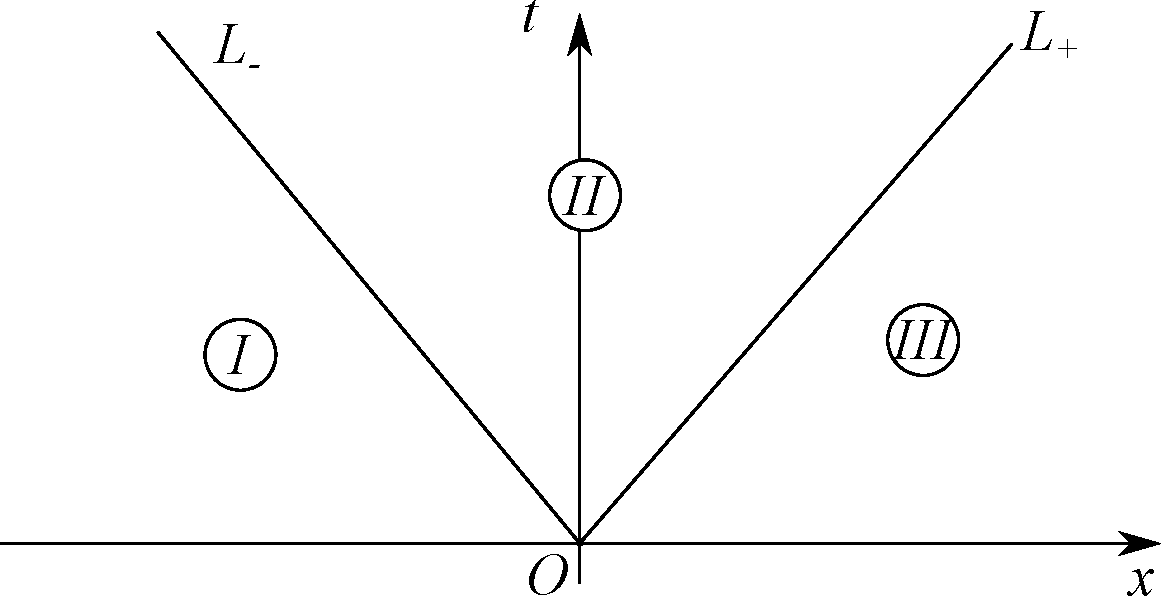
\includegraphics[width=0.5\textwidth]{../img/flow_vacuum_char_plane}
	\caption{Характеристическая плоскость для нестационарной одномерной задачи истечения газа в вакуум: $I$ -- зона невозмущенного течения; $II$ -- зона возмущенного течения; $III$ -- зона вакуума}
	\label{fig:problem_3_characteristic_plane}
\end{figure}




Поскольку течение газа в зоне $II$ граничит с невозмущенным газом в зоне $I$ вдоль линии $L_-$, то течение в зоне $II$ является простой волной или волной Римана. Для простой волны один из инвариантов Римана является глобальной константой. В данной задаче правый инвариант $r$ является постоянным в зоне $I$, поэтому он по семейству характеристик 
\[
C_+:\quad\od{x}{t} = v + c
\]
распространяется в зону $II$:
\begin{equation}
\label{eq:problem_3_r}
\left.\left(v+\frac{2 c}{\gamma-1}\right)\right|_{II} = \frac{2 c_0}{\gamma-1}
\end{equation}

Из точки $(0,0)$ на характеристической плоскости $\argtxo$ выходит веер характеристик -- центрированная волна разрежения (зона $II$). В нем вдоль семейства характеристик
\begin{equation}
	\label{eq:problem_3_Cminus_char_dfn}
C_-:\quad \od{x}{t} = v-c
\end{equation}
сохраняется инвариант $s$: 
\[
\left.\left(v-\frac{2c}{\gamma-1}\right)\right|_{II}=A\left(\frac{x}{t}\right). 
\]

Так как в области $II$ семейство характеристик $C_-$ являются прямыми линиями (см. теорию), выходящими из точки $(0,0)$, то 
уравнение характеристик  $C_-$ (\ref{eq:problem_3_Cminus_char_dfn}) в области $II$ интегрируется к виду:
\begin{equation}
\label{eq:problem_3_Cminus_char}
x = (v-c) t.
\end{equation} 

Из уравнений (\ref{eq:problem_3_r}) и (\ref{eq:problem_3_Cminus_char})  следуют формулы:
\[
v = \frac{2}{\gamma+1}  \left( c_0 + \frac{x}{t} \right),\quad 
c = \frac{2}{\gamma+1}  \left( c_0 - \frac{\gamma-1}{2}\frac{x}{t} \right).
\]

Полученные выражения используются для нахождения зависимостей $\rho\argtxo$, $p\argtxo$, $T\argtxo$ с помощью соотношений (\ref{eq:solution_r_wave}) и калорического уравнения состояния (\ref{eq:polytrop_dfn}) (найдите их). Найдите уравнения линий $L_-$ и $L_+$ и определите скорость распространения волны разрежения и скорость истечения газа в вакуум. Сравните максимальную скорость истечения в вакуум в нестационарном и в стационарном случаях.

\subsection{Задачи для самостоятельного решения}

\begin{problems}
	
	\item 
	Пользуясь методом характеристик, повторить вывод инвариантов Римана и характеристических направлений на основе изоэнтропического приближения одномерной газовой динамики.
	
	\item 
	Покажите, что центрированные волны Римана дают все автомодельные решения уравнений газовой динамики.	
	
	\item 
	Вывести формулы для аналитического решения для $r$- и $s$-волны Римана (\ref{eq:solution_r_wave}), (\ref{eq:solution_l_wave}).

	\item 
	Доказать утверждение, что всякое непрерывное течение, примыкающее к зоне постоянного течения, есть волна Римана.
	
	
	
	
	\item 
	В цилиндр, заполненный покоящимся воздухом с параметрами $v_0 = 0$, $\rho=\rho_0$, $p=p_0$, вдвигается поршень с постоянным ускорением $a$. Найти момент возникновения ударной волны $t^*$.
	
	\item
	Определить закон движения поршня площадью $S$ и массой $m$, выталкиваемого газом с начальными параметрами $v_0=0$, $p_0$, $\rho_0$ в вакуум (см. иллюстрацию).

	\begin{figure}[h!]
		\centering
		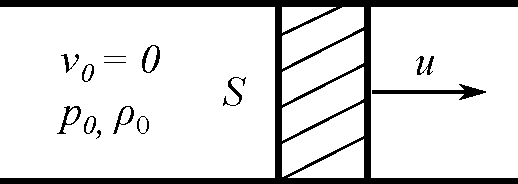
\includegraphics[width=0.5\textwidth]{../img/piston_u.pdf}
	\end{figure}
	
	\item 
	Из трубы, заполненной при $x>0$ газом с параметрами  $v_0=0$, $p_0$, $\rho_0$, начинает выдвигаться поршень с постоянной скоростью $u$. Определить движение газа.

\end{problems}

\end{document}